Descrição da interface de criação de cenários e alguns exemplos do que pode ser criado com ele.

\subsection{A ferramenta}

\subsection{Criando um cenário básico}

\subsection{Exemplos}

\begin{figure}[H]
	\centering
	\caption{Cenário 1}
	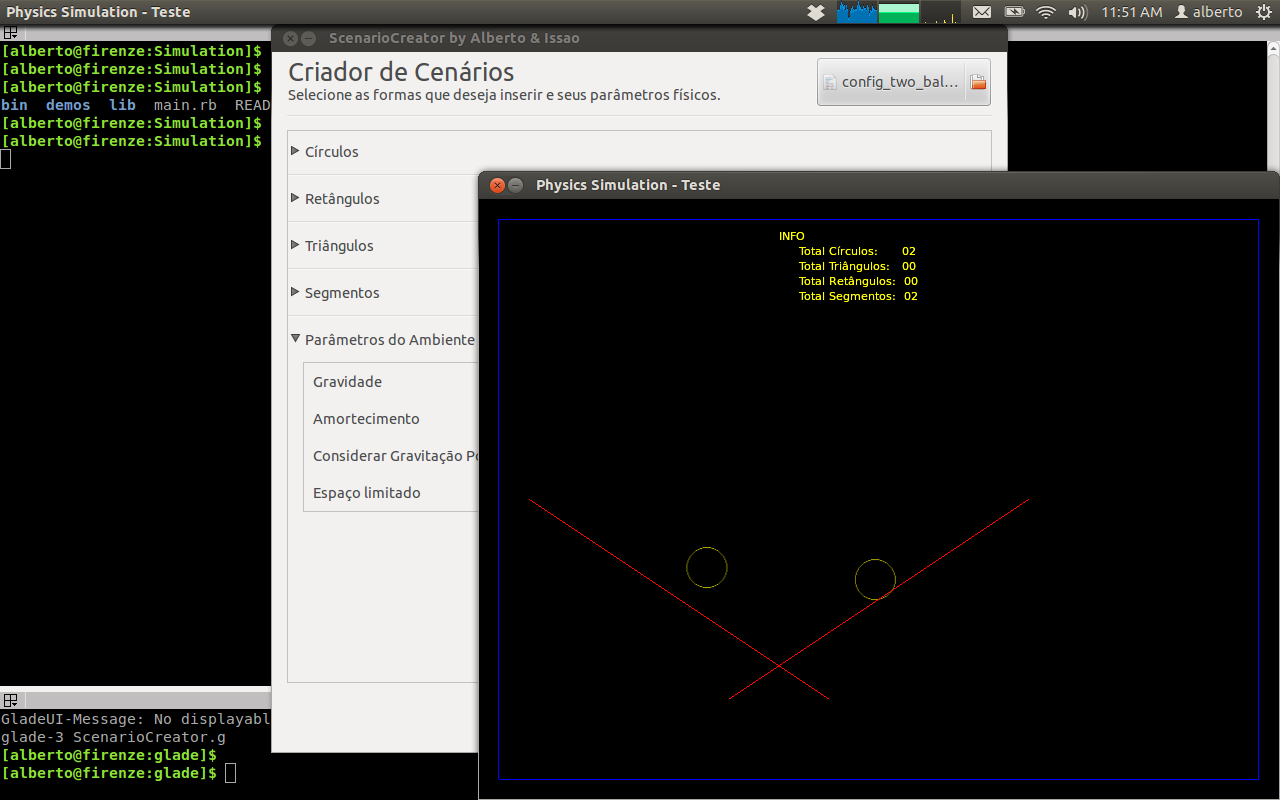
\includegraphics[scale=0.3]{images/cenario-two-balls.png}
	\hspace{0.5cm}
\end{figure}  

  \begin{figure}[H]
	  \centering
	  \caption{Cenario 2}
    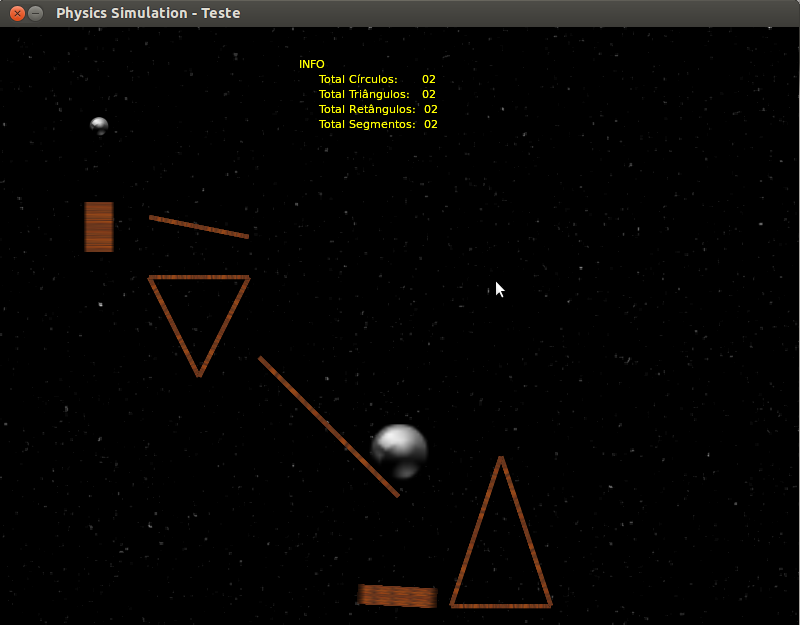
\includegraphics[scale=0.4]{images/cenario-todos.png}
  \end{figure}

  \begin{figure}[H]
	  \centering
	  \caption{Cenario 2 - Raio-X}
    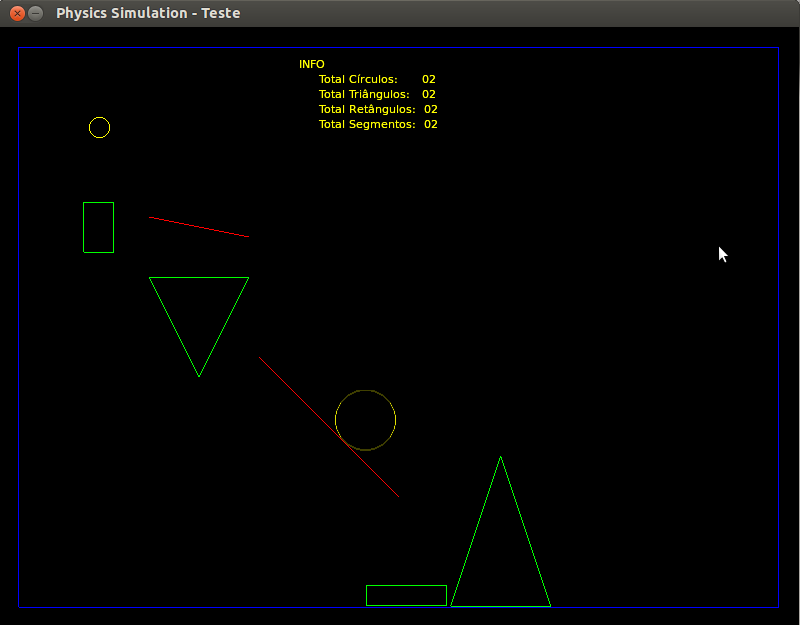
\includegraphics[scale=0.4]{images/cenario-todosE.png}
  \end{figure}

  \begin{figure}[H]
	\centering
	\caption{Cenário Gravitacão 1}
    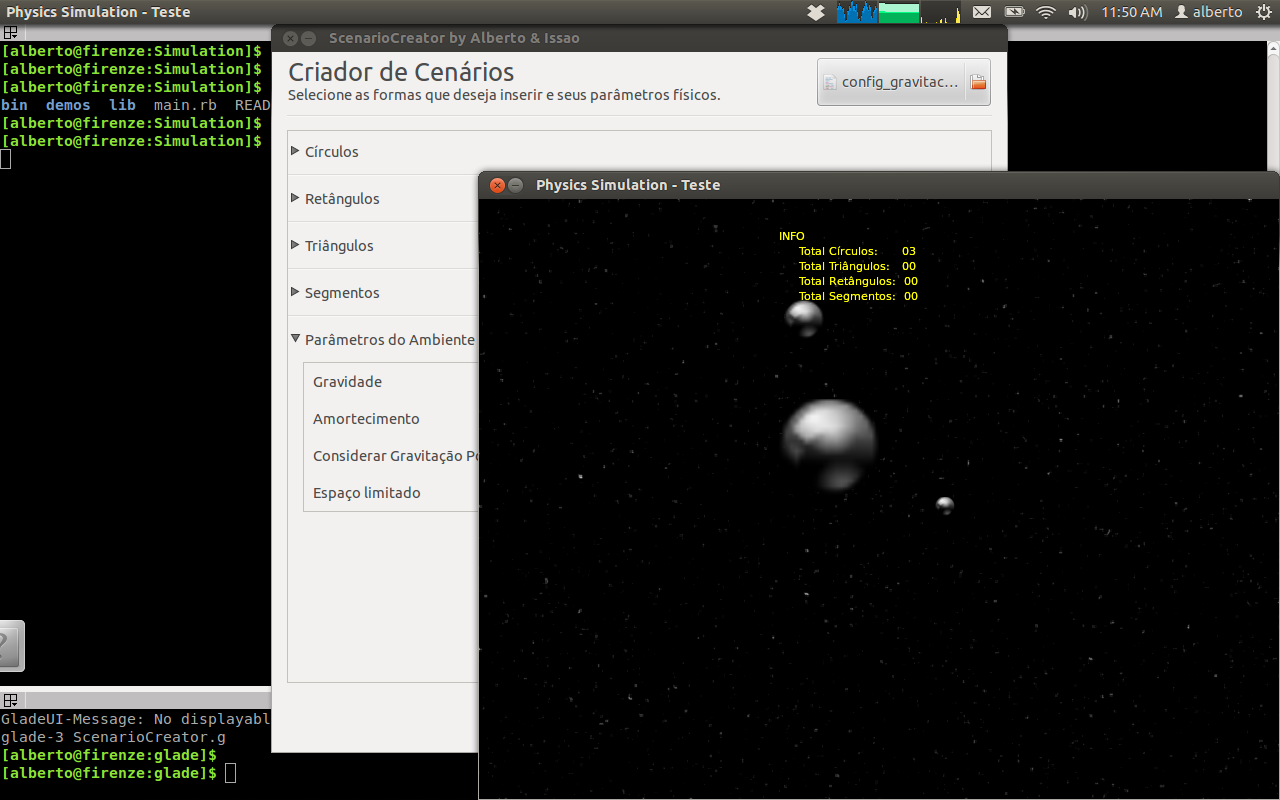
\includegraphics[scale=0.4]{images/cenario-gravitacao-2.png}
    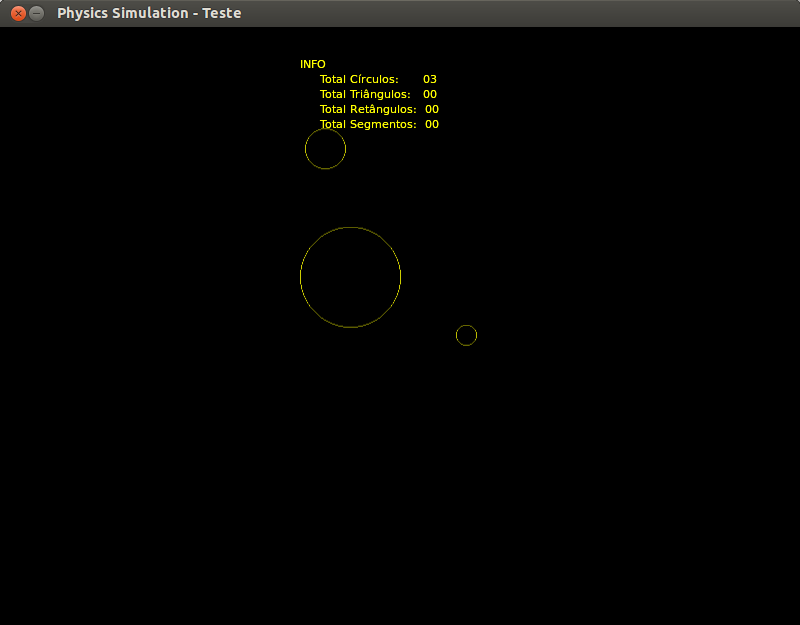
\includegraphics[scale=0.4]{images/cenario-gravitacao.png}
  \end{figure}

  \begin{figure}[H]
	\centering
	\caption{Cenário Gravitacão 2}
    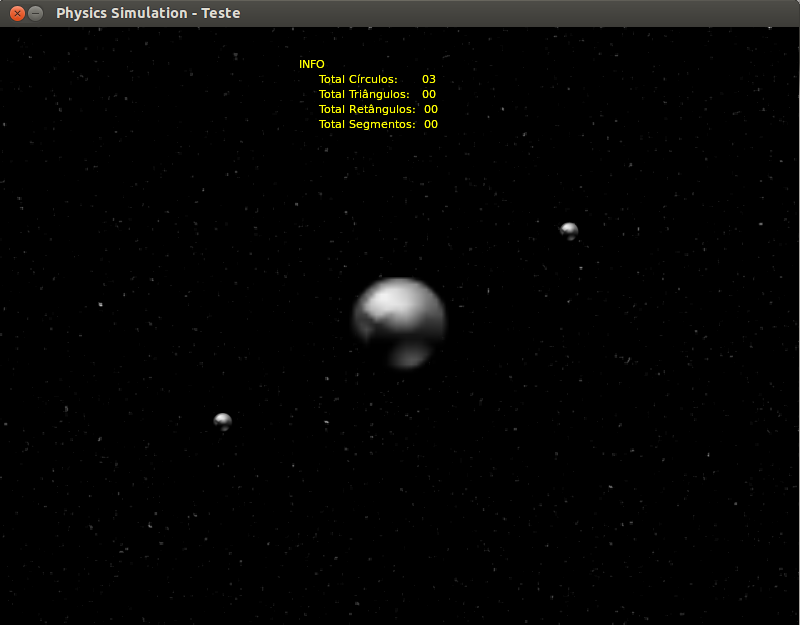
\includegraphics[scale=0.4]{images/cenario-gravitacao-4.png}
    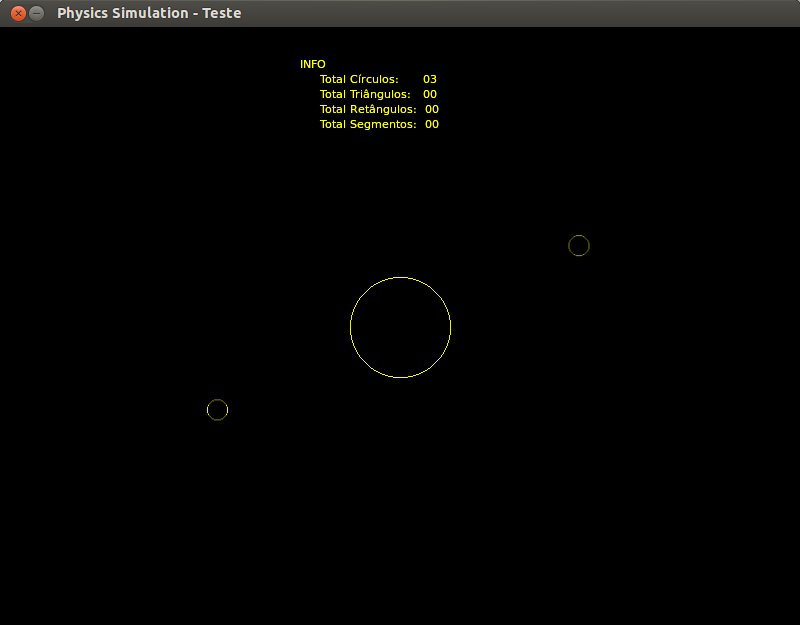
\includegraphics[scale=0.4]{images/cenario-gravitacao-3.png}
  \end{figure}

\subsection{Arquivos de configuração}
As propriedades físicas do cenário e de cada objeto ficam guardadas em arquivos *.config e podem ser modificadas...

\subsection{Pontos de modificação}
Apesar de utilizar o Chipmunk, o Physimulation possui pontos do código que podem ser modificados de acordo com o comportamento físico que deseja-se obter, o que pode ser interessante para o aluno de computação. \\

Tais pontos são... \\

Além disso, no próprio Chipmunk há trechos de código que o aluno poderá modificar e observar rapidamente mudanças na simulação. Exemplos: ...



